\section{Описание}

Имея на руках датасет с котировками акций американских компаний, попробуем смоделировать цену акций Apple на момент открытия биржи. Рассмотрим 3 различных модели регрессии и проанализируем, какие из них лучше всего справляются с задачей. Разделим данные котировок в отношении 7:3, при этом обучим модель на 70\% данных.

{\bfseries Poisson Regression.}

Пуассоновская регрессия - обобщённая форма модели линейной регрессии. Предполагается, что оцениваемая величина $Y$ распределена по Пуассоновскому закону($Y~P(\lambda)$) и что логарифм от математического ожидания $Y$ может быть представлен в виде линейной комбинации некоторых параметров $\theta$, поэтому она также называется линеарифметической: $log(E(Y|x))=log(exposure)+\theta x$.

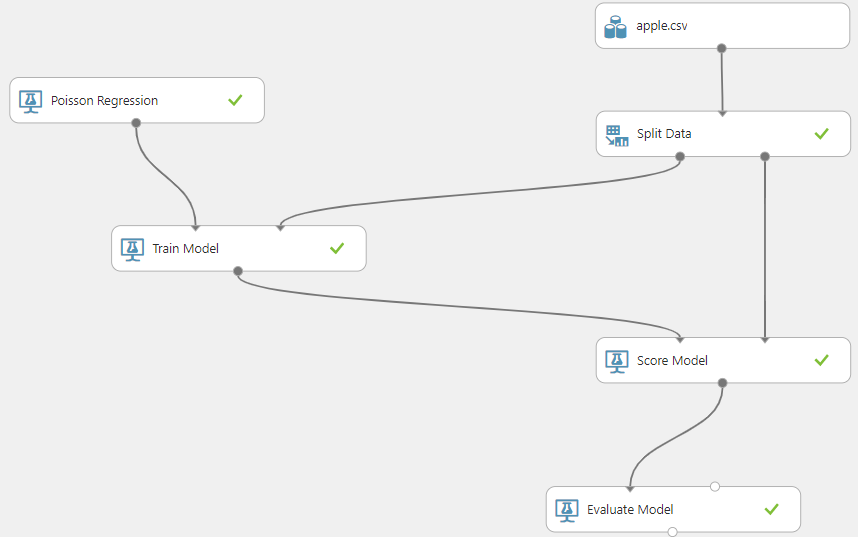
\includegraphics[width=0.7\linewidth]{src/pics/poisson2.png}
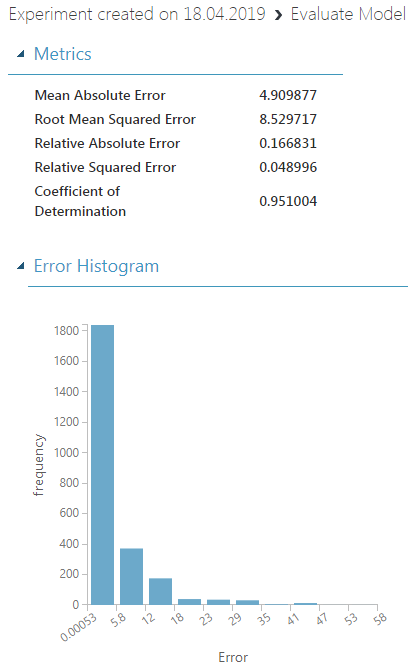
\includegraphics[width=0.3\linewidth]{src/pics/poisson1.png}

Распределение ошибки похоже на Пуассоновское, и сама величина ошибки достаточно велика. Взглянув на распределение признака Open всего датасета, видим:
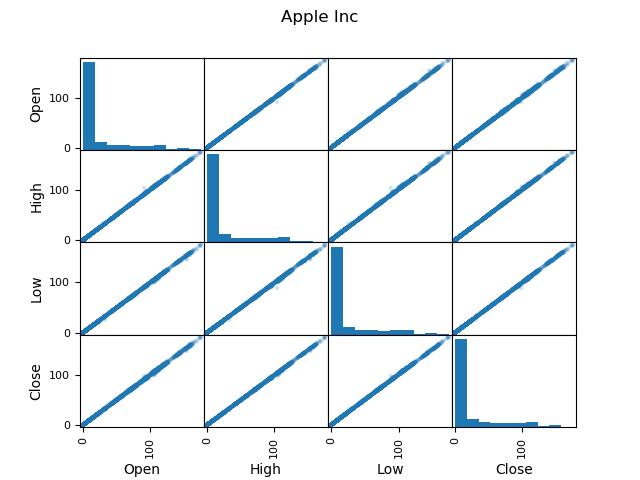
\includegraphics[width=0.8\linewidth]{src/pics/aapl.png}

Распределение не похоже на Пуассоновское, следовательно, в данном случае Пуассоновская не позволяет добиться высокой точности. Построив зависимость предсказываемой величины от предсказанной, можно в этом убедиться:

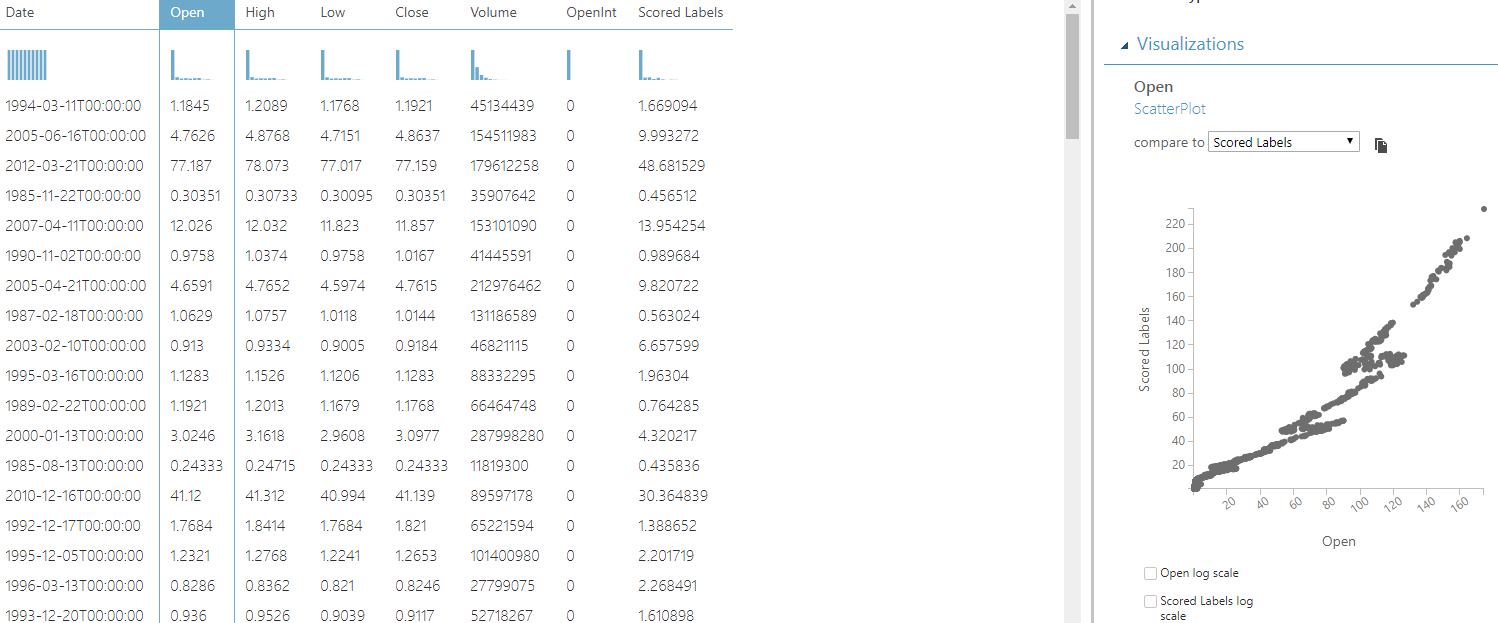
\includegraphics[width=1\linewidth]{src/pics/poisson3.png}

{\bfseries Neural Network Regression.}

Регрессия на основе нейронных сетей - адаптирование нейронных сетей, решающих сложные задачи глубокого обучения или распознавания изображений, к задачам регрессии. Любой класс статистической модели может быть представлен в виде нейронной сети, если она использует адаптивные веса и может апроксимировать нелинейные функции на входе. Эта модель может помочь тогда, когда традиционные алгоритмы регрессии не справляются с задачей.

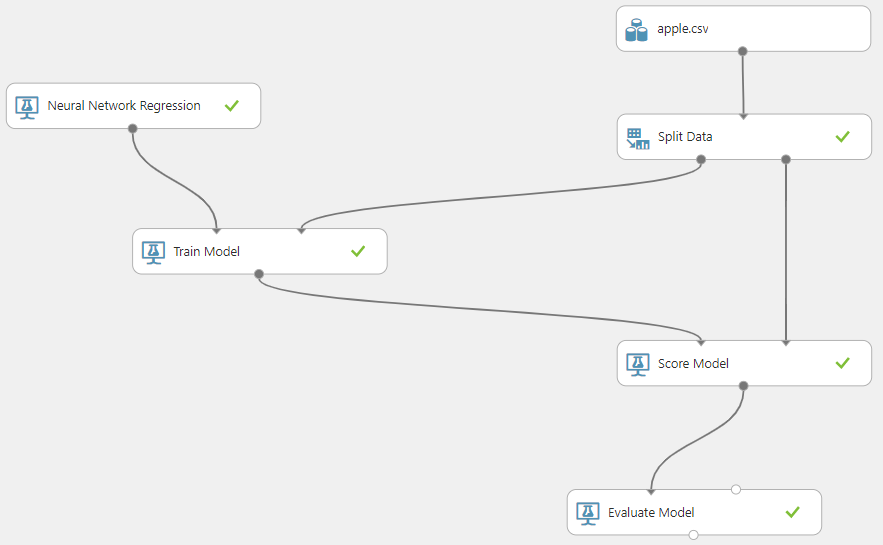
\includegraphics[width=0.7\linewidth]{src/pics/neural2.png}
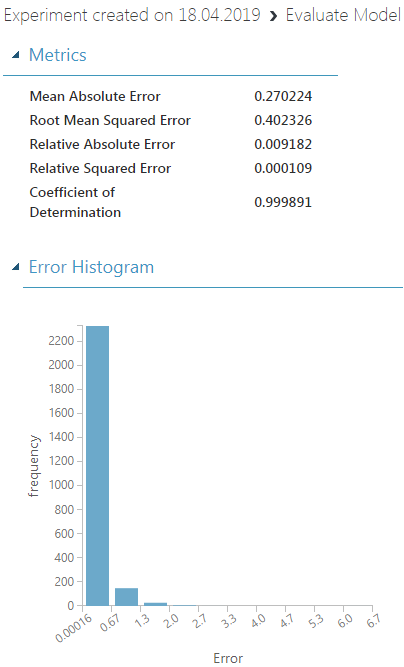
\includegraphics[width=0.3\linewidth]{src/pics/neural1.png}

В отличие от Пуассоновской регрессии, ошибка значительно меньше, что подтверждается на графике зависимости признаков:

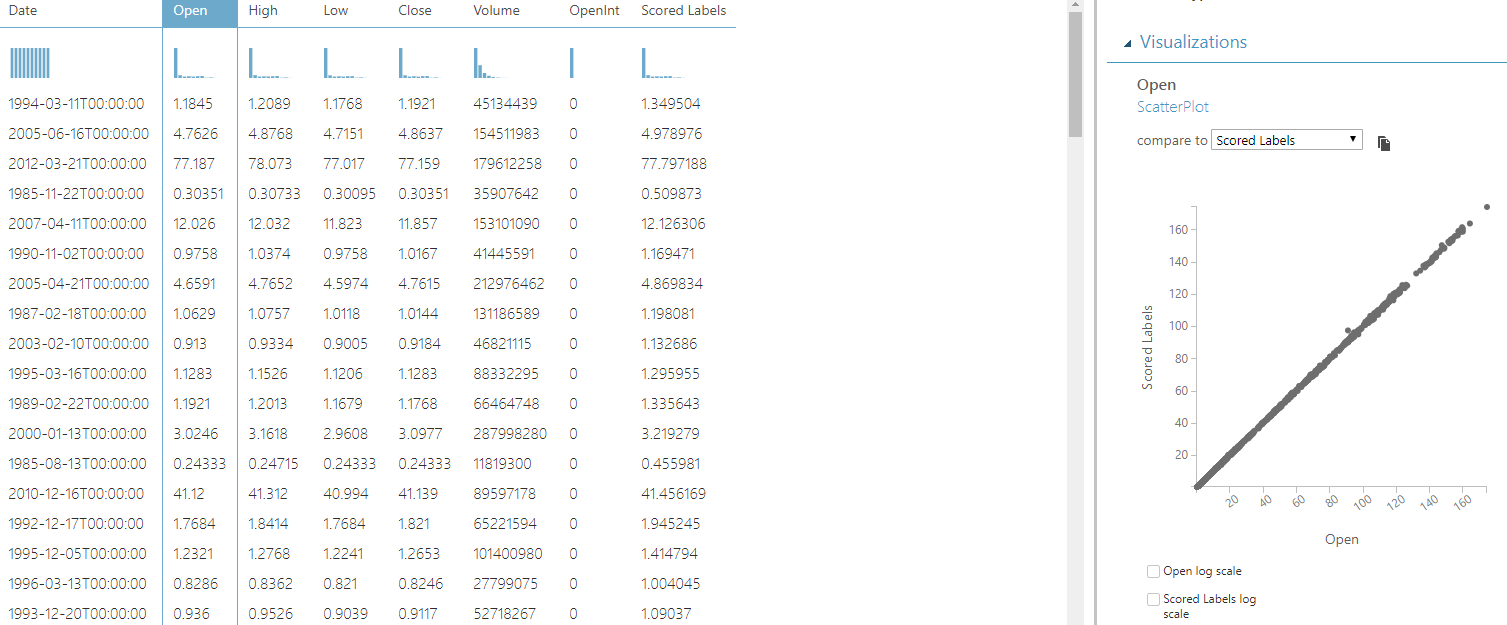
\includegraphics[width=1\linewidth]{src/pics/neural3.png}

Тем не менее, среднее отклонение составляет 0.27\$, а это около 17,26 рублей по текущему курсу. Погрешность достаточно высока, но хотя бы не Пуассон.

{\bfseries Linear Regression.}

Линейная регрессия -  используемая в статистике регрессионная модель зависимости одной (объясняемой, зависимой) переменной $y$ от другой или нескольких других переменных (факторов, регрессоров, независимых переменных) $x$ с линейной функцией зависимости. Модель линейной регрессии является часто используемой и наиболее изученной в эконометрике(наука, изучающая количественные и качественные экономические взаимосвязи с помощью математических и статистических методов и моделей). С эконометрической точки зрения более важное значение имеет линейность по параметрам, чем линейность по факторам модели.

В случае акций Apple можно сделать вывод, что данная модель подходит лучше всего, так как необходимые нам признаки линейны отонсительно друг друга. Построим данную модель:

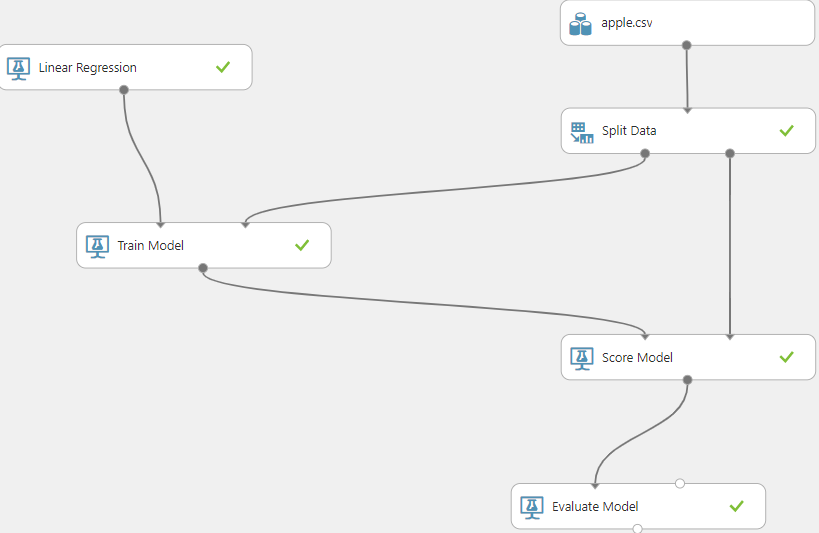
\includegraphics[width=0.7\linewidth]{src/pics/linear2.png}
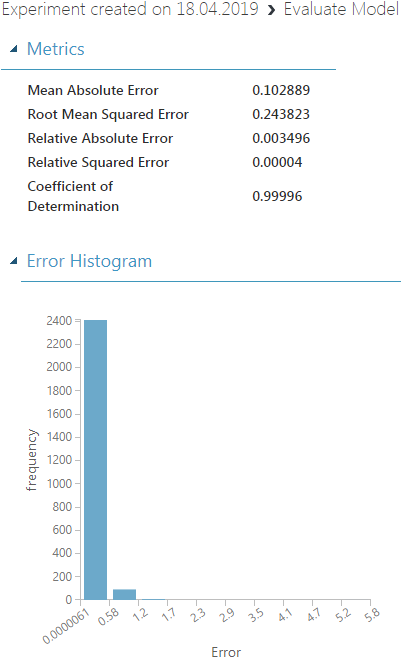
\includegraphics[width=0.3\linewidth]{src/pics/linear1.png}

В сравнении с нейронной сетью, ошибка стала более чем в 2 раза меньше: 0.1\$. Благодаря этому график зависимости предсказываемой величины от предсказанной будет похож на линейную функцию с углом наклона $\dfrac{\pi}{4}$:

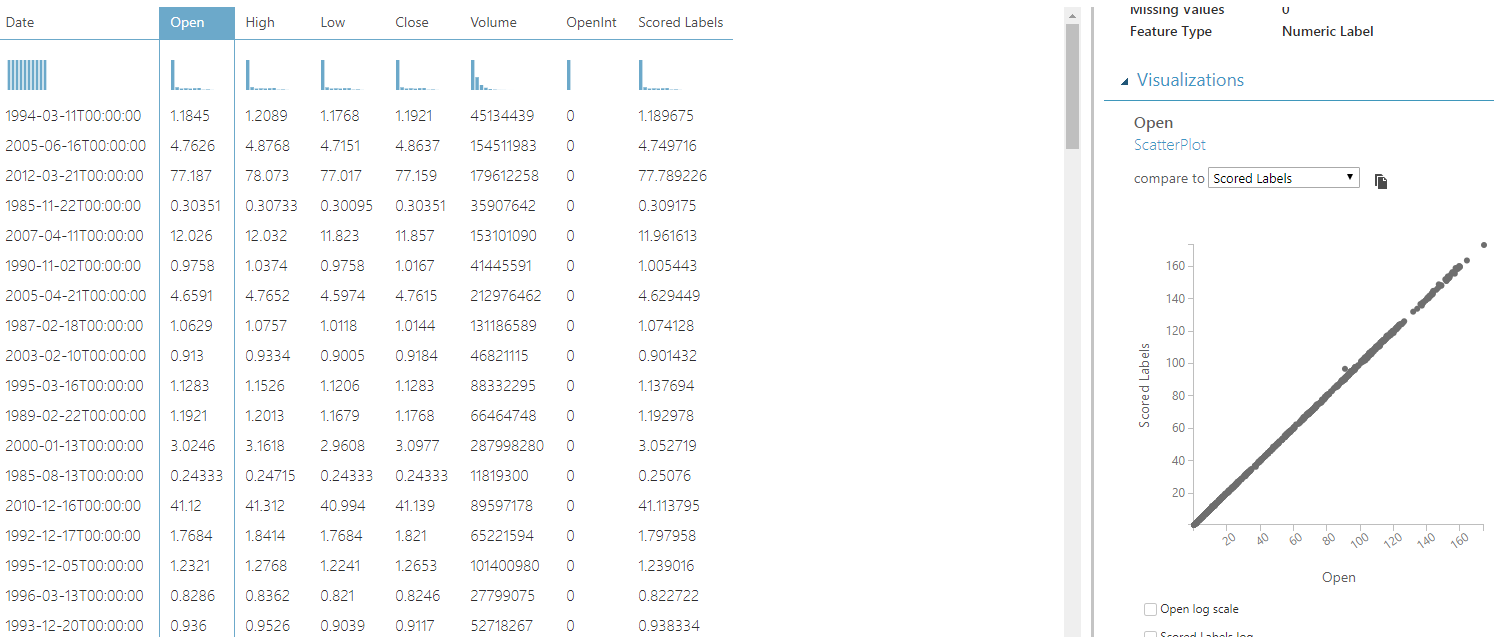
\includegraphics[width=1\linewidth]{src/pics/linear3.png}

Сравнив работу 3-х различных моделей регрессии, можно сделать вывод, что наиболее подходящей для решения задач является именно линейная модель. К сожалению, это утверждение верно не для всех котировок акций. В большинстве случаев зависимость признаков друг от друга линейная, но это не есть правило. Таким образом, задача предсказания котировок акций достаточно сложна и характеризуется не только данными о предыдущих ценах, но и другими зависимостями.